\documentclass[12pt]{../SOP4_alpha}\usepackage[]{graphicx}\usepackage[]{xcolor}
% maxwidth is the original width if it is less than linewidth
% otherwise use linewidth (to make sure the graphics do not exceed the margin)
\makeatletter
\def\maxwidth{ %
  \ifdim\Gin@nat@width>\linewidth
    \linewidth
  \else
    \Gin@nat@width
  \fi
}
\makeatother

\definecolor{fgcolor}{rgb}{0.345, 0.345, 0.345}
\newcommand{\hlnum}[1]{\textcolor[rgb]{0.686,0.059,0.569}{#1}}%
\newcommand{\hlstr}[1]{\textcolor[rgb]{0.192,0.494,0.8}{#1}}%
\newcommand{\hlcom}[1]{\textcolor[rgb]{0.678,0.584,0.686}{\textit{#1}}}%
\newcommand{\hlopt}[1]{\textcolor[rgb]{0,0,0}{#1}}%
\newcommand{\hlstd}[1]{\textcolor[rgb]{0.345,0.345,0.345}{#1}}%
\newcommand{\hlkwa}[1]{\textcolor[rgb]{0.161,0.373,0.58}{\textbf{#1}}}%
\newcommand{\hlkwb}[1]{\textcolor[rgb]{0.69,0.353,0.396}{#1}}%
\newcommand{\hlkwc}[1]{\textcolor[rgb]{0.333,0.667,0.333}{#1}}%
\newcommand{\hlkwd}[1]{\textcolor[rgb]{0.737,0.353,0.396}{\textbf{#1}}}%
\let\hlipl\hlkwb

\usepackage{framed}
\makeatletter
\newenvironment{kframe}{%
 \def\at@end@of@kframe{}%
 \ifinner\ifhmode%
  \def\at@end@of@kframe{\end{minipage}}%
  \begin{minipage}{\columnwidth}%
 \fi\fi%
 \def\FrameCommand##1{\hskip\@totalleftmargin \hskip-\fboxsep
 \colorbox{shadecolor}{##1}\hskip-\fboxsep
     % There is no \\@totalrightmargin, so:
     \hskip-\linewidth \hskip-\@totalleftmargin \hskip\columnwidth}%
 \MakeFramed {\advance\hsize-\width
   \@totalleftmargin\z@ \linewidth\hsize
   \@setminipage}}%
 {\par\unskip\endMakeFramed%
 \at@end@of@kframe}
\makeatother

\definecolor{shadecolor}{rgb}{.97, .97, .97}
\definecolor{messagecolor}{rgb}{0, 0, 0}
\definecolor{warningcolor}{rgb}{1, 0, 1}
\definecolor{errorcolor}{rgb}{1, 0, 0}
\newenvironment{knitrout}{}{} % an empty environment to be redefined in TeX

\usepackage{alltt}
%\documentclass[12pt]{~/github/SOPs/SOP_Template/SOP}

\usepackage[english]{babel}
%\usepackage{blindtext}
%\usepackage{lipsum}

%\documentclass{article}

\usepackage{natbib}

\title{Compost Maturity}
\date{1/27/2024}
\author{Marc Los Huertos}
\approved{Los Huertos}
\ReviseDate{\today}
\SOPno{37b~v0.92}
\IfFileExists{upquote.sty}{\usepackage{upquote}}{}
\begin{document}
%\SweaveOpts{concordance=TRUE}

\maketitle

\section{Scope and Application}

\NP The Solvita Compost Maturity Test is a unique procedure using two test probes to simultaneously measure CO$_2$ and NH$_3$, the two most prominent gases indicating activity and stability of compost.

\NP This test is widely-recognized worldwide for validating compost maturity.

\NP This easy-to-use application requires a small sample placed in the incubation jars and the results are read after 4-hrs of exposure.  The basic kit offers a Solvita color chart to determine the level of activity from which a Maturity Index is calculated using guidelines provided in the manual.

\NP 

\NP Numerous studies\ldots \citep{vargas2005assessing}.

\section{Acknowledgements}

\NP This SOP is based on the Solvita Field Test Kit Manual \citep{solvita2014}, version 8.

\section{Definitions}

\begin{description*}

\item[Compost] Compost is a mixture of organic residues that have been piled, watered, and have undergone thermophilic and mesophilic decomposition.

\item[Compost Maturity] Compost maturity is the degree of stability of the compost product and the degree to which it is free of phytotoxic (plant-toxic) compounds. Figure~\ref{fig:CompostMaturity} shows the relationship between compost maturity and the composting process.

\begin{figure}[htbp]
   \centering
   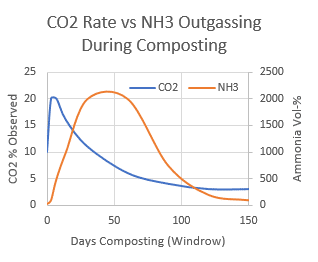
\includegraphics[width=5in]{graphics/CompostCO2NH3} 
   \caption{Compost Maturity}
   \label{fig:CompostMaturity}
\end{figure}



\item[Maturity Index] The Maturity Index is a numerical value that is calculated from the CO$_2$ and NH$_3$ readings. The Maturity Index is a relative measure of the degree of stability of the compost. The higher the Maturity Index, the more stable the compost. The Maturity Index is calculated using the following formula:

\end{description*}

\section{Biases and Interferences}

\NP Biases and interferences can come from...



\section{Health and Safety}

%NP \lipsum[2]


\section{Personnel \& Training Responsibilities}

%\NP \lipsum[1]

Students using this SOP should be trained for the following SOPsa:

\begin{itemize*}
  \item SOP1
  \item SOP2
\end{itemize*}

\section{Required Materials}

\begin{itemize*}
  \item Test Soils
  \item \# XX Seives (3/8" or 10 mm)
  \item Solvita Jars
  \item Individually wrapped CO$_2$ \& NH$_3$ Probes (must remain refrigerated) 
  \item DCR Field Test Unit (with 9 volt battery)
  \item AWS digital scale (field) or Ohaus digital scale (lab)
\end{itemize*}

\section{Estimated Time}

\NP This will take 20 minutes to collect and prepare compost sample. An equalibrium stage ranges from 1 to 24 hours depending on conditions. The incubation requires 4 hours. Finally, an additional 10 minutes is needed to read the probes for a total of 5.5 to 28.5 hours.

\section{Sample Collection, Preservation, and Storage}

\subsection{Obtain and Prepare Sample}

\NP Take several grab samples to prepare a compost by mixing all sub-samples respresenative of the enre compose. Remove larg weed chips and other objects. A 3/8" (10 mm) seive is recommended before laoding jar.

\NP Check moisture content of sample using squeeze test. Squeeze a handful of compost and release. Water should appear between fingers, but not drip out. Adjust water content if needed. Allow compost to equilibrate for 24 hours.

\NP If compost is warm or frozen, let it equilibrate to room temperature for 24 hours before testing.

\section{Procedure}

\NP Seive compost to remove large particles.

\NP Carefully fill the Solvita jar to the fill lines. To get the proper density tap the jar gently while filling to fill line. Optionally, the proper weight in grams per jar corresponding to actual field density is found in the Table~\ref{tab:jarweight}.

\begin{table}[ht]
\caption{Compost weight per jar adjusted for actual field density.}
\label{tab:jarweight}
\centering
\begin{tabular}{rrr}
  \hline
 \textbf{lbs/yr3} & \textbf{kg/m3} & \textbf{g/jar} \\ 
  \hline \hline
  500   & 300   & 30 \\
  800   & 475   & 50 \\
  1,000 & 600   & 60 \\
  1,200 & 700   & 70 \\ \hline
\end{tabular}
\end{table}


\NP Let the sample ``air-out" briefly in the jar for up to one-hour prior to starting the test. If the sampl was take directly from a very hot or frozen pile, it is advisable to allow it to stand for 24 hours before starting the test. 

\NP The Solvita maturity method requires two tests carried out simultanious in the same 4-hour period. Tear open both the pouches marked ``High CO$_2$" and ``Ammonia" and carefully remove each probe and avoid touching the gel surface. The gel in the proble is color-coded: the carbon dioxide probe is purple and the ammonia probe is yellow. Once the pouch is open, the test should be started immediately. 

\begin{figure}[htbp]
   \centering
   \includegraphics[width=2.5in]{graphics/Solvita_Paddle_image} 
   \caption{Solvita Probes, Ammonia (NH$_3$) (left paddle) and Carbon Dioxide (CO$_2$) (right paddle).}
   \label{fig:Probes}
\end{figure}


\NP Carefully insert both probes into the compost without allowing compost to touch the gel surface. Push the probes so the bottom of the probe hits the jar's bottom. Do not jostle the composite or allow dust to coat the surface of the probe. 

\NP Screw on lid tightly and allow to incubate out of direct sunlight -- and wait 4 hours. Record temperature and try to keep the jars at a constant temp for the duration of the test, between 20-25\textdegree C (68-77\textdegree F).

\NP Remove lid after 4 hours and remove the probes. 

\NP Read the probes immediately after removing from the jar.


\subsection{Reading the Results}

\NP Turn on DCR Field test unit and insert probe to get CO$_2$ and NH$_3$ color. The probe must go into the DCR with gel side up press the read button. 

\NP Insert the NH3 probe into the DCR and press the read button. Compare color to the visual color key. Record the NH3 reading.

\NP If the DCR does not work, Compare the color of the gel to the color chart, finding the closest match. Record the CO2 and NH3 readings.

\begin{figure}[ht]
\centering
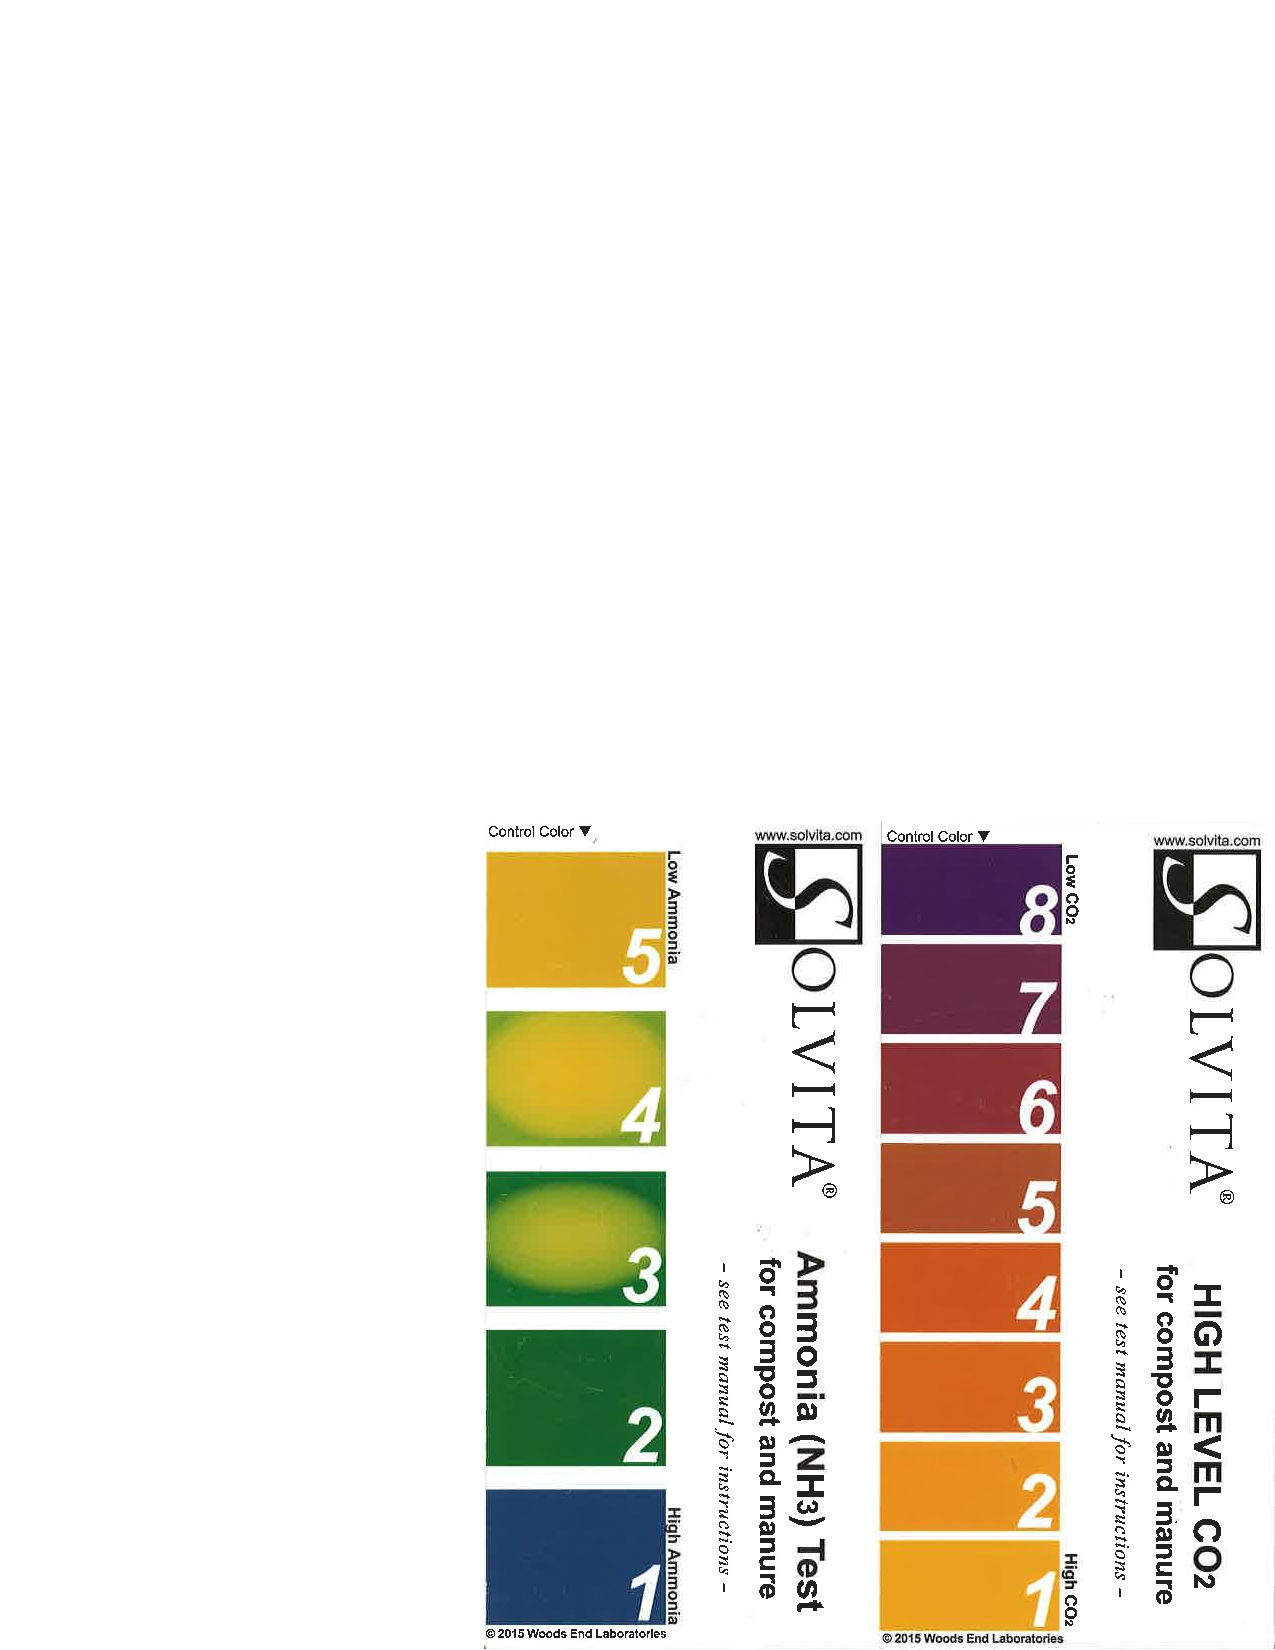
\includegraphics[width=0.70\textwidth]{graphics/Solvita_Color_Chart_NH3_CO2}
\caption{Interpretation of compost maturity index.}
\label{fig:CompostMaturity}
\end{figure}

\subsection{Clean Up}

\NP Discard compost sample and probe in an appropriate manner.

\NP Wash the Solvita jar with water and dry for reuse. Label jar top with event to track the number of times the jar has been used. Disscard the jar after 4 uses.

\section{Data Analysis and Calculations}

\NP Calculate the maturity index using the following formula.

\begin{table}[ht]
\caption{Compost weight per jar adjusted for actual field density.}
\label{tab:jarweight}
\centering
\begin{tabular}{lll}
  \hline
 \textbf{lbs/yr3} & \textbf{kg/m3} & \textbf{g/jar} \\ 
  \hline \hline
  500   & 300   & 30 \\
  800   & 475   & 50 \\
  1,000 & 600   & 60 \\
  1,200 & 700   & 70 \\ \hline
\end{tabular}
\end{table}

%\begin{equation}
%MI = \frac{CO2 \times 0.5 + NH3 \times 0.5}{100}
%\end{equation}


\subsection{Compost Maturity Index}

\NP See Figure! 1 below for interpretation:

\section{Applications of Results}

\subsection{Status and Conditions of Compost Processes}

\begin{figure}[ht]
\centering
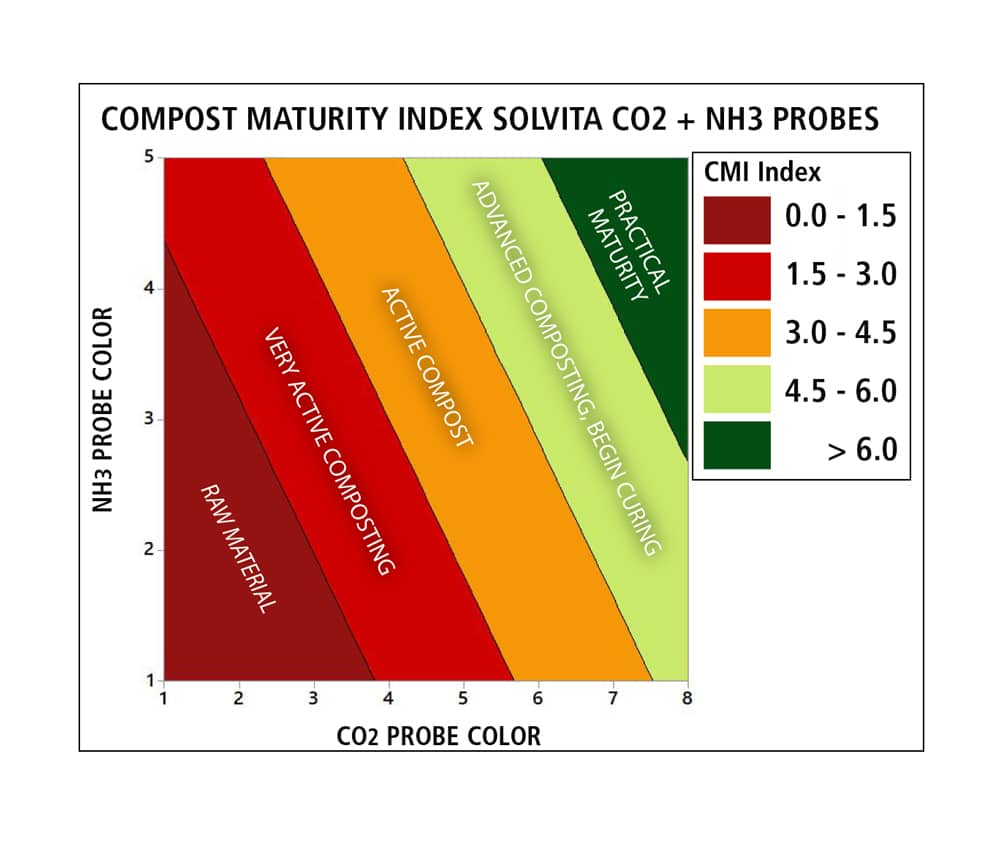
\includegraphics[width=0.75\textwidth]{graphics/Solvita_CMI_Calculator}
\caption{Interpretation of compost maturity index.}
\label{fig:fig1}
\end{figure}

\subsection{Managing Aeration Sufficiency}

\subsection{Selecting Best Use of Composed Based on Maturity}


\subsection{Ammoiniua Emissions of Mantures \& Composts}

\section{QC/QA Criteria}

\NP The probe show Lot No. and Expiration Dates on the package. Solvita kits are pre-calibrated and packaged for the highest quality prior to shipping. The sealed probes should be the "Control Color" when the foil pack is opened (see color chart).  Shelf-life is improved by refrigeration. Do not allow gels to freeze. 

\NP The plastic jars may be reused 4 times, the discarded. 

\NP If the foil packs are damaged or the jar is cracked then the test may not work properly.

\NP A sample that is too dry may give a false postive maturiety test (although goty ammonia is still volatile).

\section{Trouble Shooting}

\begin{table}[ht]
\centering
\caption{Trouble Shooting Guide}
\begin{tabular}{p{5cm}p{5cm}p{5cm}} \hline
\textbf{Problem} & \textbf{Cause} & \textbf{Solution} \\ \hline \hline
Compost is fresh but test results indicate ``mature"& 
Compost is too dry & 
Add water to compost and retest \\


\end{tabular}
\end{table}

\section{References}

\bibliographystyle{apalike}
\bibliography{references}

%\NP APHA, AWWA. WEF. (2012) Standard Methods for examination of water and wastewater. 22nd American Public Health Association (Eds.). Washington. 1360 pp. (2014).


\end{document}
